\chapter{ Description of the model \label{ch:numero_uno}}
\section{An invitation to Signed Distance Fields}
The use of signed distance fields (SDFs) to model organic sufaces
is a time honoured graphical technique used, for example, by Pixar
Animation Studios to model hair in \textit{The Incredibles} 
(see \cite{petrovic2005volumetric}). The idea is to define a 
function which represents the closest distance from the query point
to a point on the surface of the object that is to be represented. 
If the query point is outside, the SDF is positive,
the SDF is zero on the surface and negative inside. SDFs can be 
rendered within traditional graphics pipelines (such as OpenGL or Vulkan)
using raymarching, a method that takes place within shader programs and 
is therefore meshless. The formulae defining SDFs for common 2D and 3D 
shapes are easy to find online, see \cite{key}. Whilst the simulations 
herein are done using 2D SDFs, a quick 3D primer is given below.
\\
To motivate the primary mechanism by which cells will undergo mitosis 
in this thesis, we consider a toy example in which the equations for 
two spheres undergo a catastrophic topological change as one parameter 
changes. We start by considering the equations for two spheres which 
begin as coincident and move apart as the parameter $a$ becomes larger. 
In order to combine the first equation
\\
\begin{equation*}
    f_1(x,y,z) =  \sqrt{ (x+a)^2+y^2+z^2 } -r,
\end{equation*}
\\
with the second equation
\\
\begin{equation*}
    f_2(x,y,z) =  \sqrt{(x-a)^2+y^2+z^2 } - r,
\end{equation*}
\\
we require a smooth combination function. We construct the combined SDF
using what is called a ``union" in the graphics community 
(see \cite{fusekvisualization}). This is the pointwise minimum 
\\
\begin{equation*}
    f_{\textrm{union}}(x,y,z) = \min(f_1(x,y,z), f_2(x,y,z)).
\end{equation*}
\\
To get smooth transition between the cells as they come apart we use 
$\textrm{smoothmin}$ which is defined by a smoothness parameter $k$, as in

\begin{equation}
    \textrm{smoothmin}(x_1, x_2) = -k \log(e^{-x_1/k} + e^{-x_2/k}).
\end{equation}

As shown in Figure \ref{fig:ToyMitosis}, we have a smooth splitting of a 
cell as the parameter $a$ ranges from $0.0$ to $5.0$. Here $r$ is the
nominal sphere radii, and $k$ is a smoothing parameter. The larger $k$ 
is, the more smoothly the two curves cling to each other. We plot the 
level-$0$ surface of the smooth union SDF using MATLAB's 
\codeword{isosurface} function. 

\begin{figure}[h]
\centering
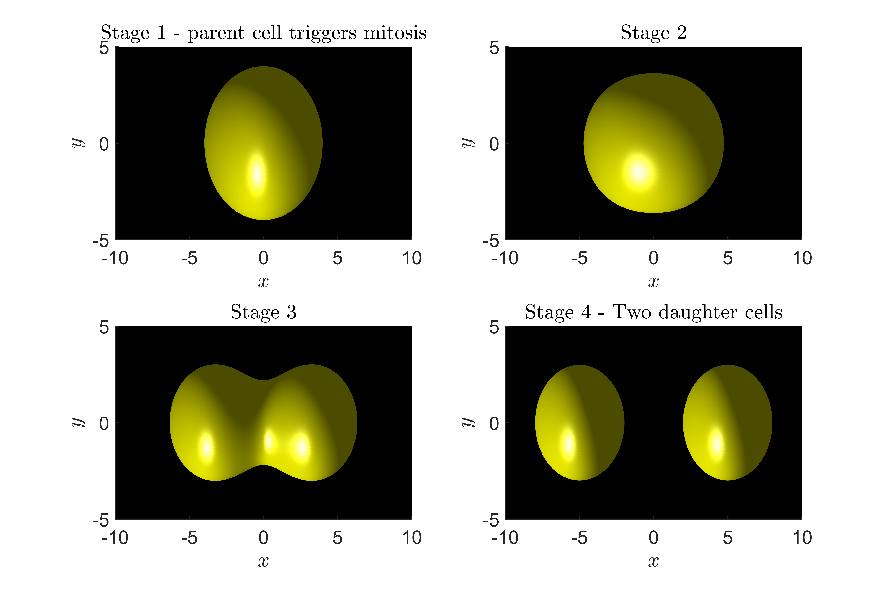
\includegraphics[width=1\textwidth]{chapter1/figures/CellDivisionDemo.pdf}
\caption{A toy example of mitosis using implicit equations for spheres in 3D. 
Stage 1 is $a= 0.0$, Stage 2 is $a= 1.67$, Stage 3 is $a=3.33$, Stage 4 is $a = 5.0$}
\label{fig:ToyMitosis}
\end{figure}
\filbreak
It is also possible to get the intersection of two SDFs using a $\textrm{smoothmax}$ function.

\section{Modeling yeast cells with ellipses}
A signed distance field for the ellipse is used to model Baker's yeast cells.
An ellipse centered at the origin with semi-major dimension $a$ (the $x$ intercept) and
semi-minor dimension $b$ (the $y$ intercept) has an SDF given by
\begin{equation*}
    f(x,y) = \sqrt{ \left( \frac{x}{a} \right)^2 + \left( \frac{y}{b} \right)^2 } - 1.
\end{equation*}
This is not really a \textit{distance} field because it is 
dimensionless but it will still be called an SDF since it produces the 
elliptical shape all the same. Here is our ellipse.
\begin{figure}[h]
\centering
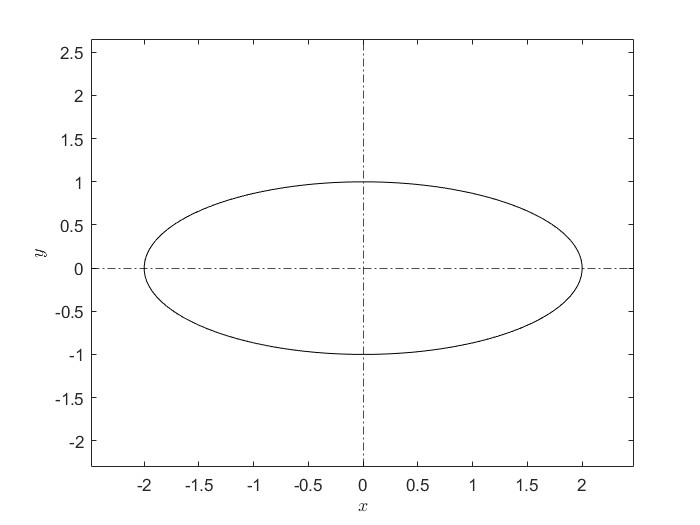
\includegraphics[width=0.5\textwidth]{chapter1/figures/ellipse_origin.jpg}
\caption{An ellipse centered at the origin with $a = 2$ and $b=1$.}
\label{fig:Ellipse_Centered}
\end{figure}
We can also translate and rotate the ellipse, using
\begin{equation*} 
    \Delta \vb{x}' = 
    \begin{bmatrix}
        \cos{\theta} & \sin{\theta} \\
        -\sin{\theta} & \cos{\theta} 
    \end{bmatrix}
    \Delta \vb{x},
\end{equation*}
where $\Delta \vb{x} = (x-x_0) \hat{\vb{i}} + (y-y_0)\hat{\vb{j}} $ and $(x_0,y_0)$ is the
center of the ellipse. We call the components of $\Delta \vb{x} = \Delta x \hat{\vb{i}} +
\Delta y \hat{\vb{j}} $ and develop the following formula
\begin{equation*}
    f(x,y) = \sqrt{ \left[\frac{ (x-x_0)\cos{\theta} + (y-y_0) \sin{\theta}}{a} \right]^2 
            +       \left[ \frac{-(x-x_0)\sin{\theta} +(y-y_0) \cos{\theta}}{b} \right]^2 } - 1.
\end{equation*}
\begin{figure}[h]
    \centering
    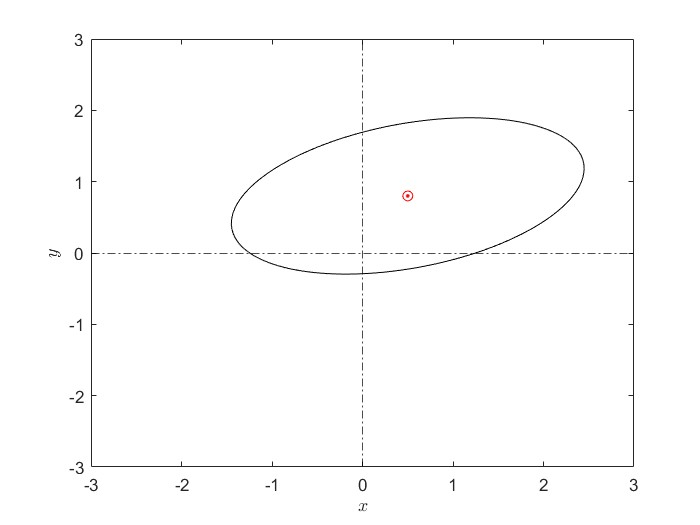
\includegraphics[width=0.5\textwidth]{chapter1/figures/ellipse_translated_rotated.jpg}
    \caption{An ellipse centered at $(0.5, 0.8)$ with $a = 2$, $b=1$ and $\theta = 15^{\circ}$.}
    \label{fig:Ellipse_Centered}
    \end{figure}
\\
Cell colonies can be built up by combining the SDFs of the individual cells 
using a cumulative $\textrm{smoothmin}$. We employ the main aspect of 
$\textrm{smoothmin}$, which is that 
\begin{equation}
    \textrm{smoothmin}(f_3, \textrm{smoothmin}(f_1,f_2)) = -k \log( \sum_{j=1}^3 e^{-f_j/k}),
\end{equation}
therefore we can accumulate smoothmins easily using
\begin{equation}
    \textrm{smoothmin}(f_1, \ldots, f_N) = -k \log( \sum_{j=1}^N e^{-f_j/k}),
\end{equation}
\begin{figure}[h]
\centering
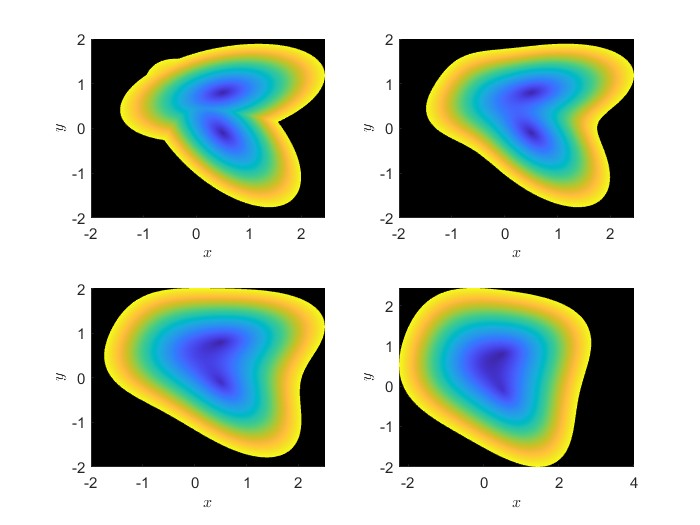
\includegraphics[width=1\textwidth]{chapter1/figures/ellipse_SDFs_blended.jpg}
\caption{Two ellipses blended with various values of $k$. 
Top left: $k= 0.005$, Top right: $k=0.2$, Bottom left: $k = 0.5$, Bottom right: $k=1.0$}
\label{fig:Ellipse_Centered}
\end{figure}


\section{Cell colony as dynamical system}
Each cell indexed $j \in \{1, \ldots N\}$ has five pieces of data which are enough to define globally the 
SDF of the cell, namely, the center coordinates $(x_j,y_j)$, the angle of orientation $\theta_j$, 
and the semi axes dimensions $a_j, b_j$. Each piece of data will be a function of time $t$. For 
the purpose of simplicity, we model each cell as two point masses $m_1 = m_2 = m$ connected by a spring 
with stiffness $K$. The point masses are located at $\vb{r}_j^{(1)}$ and $\vb{r}_j^{(2)}$ inside the ellipse 
along the major axis and symmetrically about the ellipse center. This means that the center is given by 
\begin{equation*}
    \vb{x}_j = \frac{1}{2} \left(\vb{r}_j^{(1)} + \vb{r}_j^{(2)}\right).
\end{equation*}
Fixing the semi-minor axis $b_j$, we give the semi-major axis $a_j$ by 
\begin{equation*}
    a_j = a_0||\vb{r}_j^{(1)} - \vb{r}_j^{(2)}||.
\end{equation*}
We extract the orientation angle using a two argument inverse tangent function,
\begin{equation*}
    \theta_j = \arctan(y_j^{(2)} - y_j^{(1)},x_j^{(2)} - x_j^{(1)} )
\end{equation*}

When the number of cells is fixed, the colony dynamics is modelled
using first order EOMs with two primary forces: intracellular spring force and
and intercellular contact force to void overlap. We take the assumption that 
many authors make (include reference here) which is that inertia is negligible
due to drag effects (more on this). That is the velocity is directly
proportional to the force
\begin{equation*}
\vb{v}_j^{(i)} = \frac{1}{\eta} \vb{F}_j^{(i)},
\end{equation*}
where $i \in \{1,2\}$ and $j \in \{1, \ldots, N\}$ where $\eta$ is an expression for
the drag and $\vb{F}_j^{(i)}$ is the sum of the forces acting on the $i$-th particle of
the $j$-th cell. Overall, the simulation will be begun with $V$ vertices where $V$ is a
positive power of $2$. We map from local indices $(i,j)$ to a global index $n$ using
\begin{equation*}
    n = 2(j-1) +i,
\end{equation*}
which is called ``row major order''. We then flatten the list of $x$-coordinates and 
$y$-coordinates into one state vector $\vb{X}(t)$ given by
\begin{equation*}
    \vb{X}(t) = [x_1(t), \ldots, x_V(t), y_1(t), \ldots, y_V(t)]^T,
\end{equation*}
where $(x_n,y_n)$ is the coordinate of the $n$-th vertex for $n \in \{1,\ldots,V\}$.
Note that the change in the number of cells is simulated by removing constraints
between the vertices. At the beginning of the simulation $x_1 = \cdots = x_V$ and
$y_1 = \cdots = y_V$. The first order ordinary differential equation is phrased
in terms of a mass matrix and a force function,
\begin{equation*}
    M(t,\vb{X})\frac{d \vb{X} (t)}{dt} = f(t,\vb{X})
\end{equation*}
We start by considering the spring force acting on the $n$-th particle due to the $m$-th 
particle given $n$ and $m$ are connected by springs. This is given by $\vb{F}_{nm}^{\textrm{spring}}$ as
\begin{equation*}
    \vb{F}_{nm}^{\textrm{spring}} = 
    K(|| \vb{x}_m - \vb{x}_n|| - L_{nm}) \frac{\vb{x}_m - \vb{x}_n}{|| \vb{x}_m - \vb{x}_n||},
\end{equation*}
where $K$ is a spring constant meant to represent cell elasticity, and $L_{nm}$ is the nominal length
of the spring connecting them. There are three situations regarding edge between vertex $n$ and $m$:
either they are connected by a spring with $L_{nm}>0$, they are collocated by an equality constraint
or they are disconnected. If the two masses are collocated by an equality constraint, then the 
spring force is undefined so we must omit this. We must also omit the contact force because this 
has no sense for collocated vertices. The contact force between two disconnected vertices is given as
\begin{equation*}
    \vb{F}_{nm}^{\textrm{contact}} =
    \begin{cases} 
        C\frac{\vb{x}_m - \vb{x}_n}{|| \vb{x}_m - \vb{x}_n||}, \ \textrm{if} \ || \vb{x}_m - \vb{x}_n|| \leq d \\
        \vb{0}, \ \textrm{if} \ || \vb{x}_m - \vb{x}_n|| > d,
    \end{cases}
\end{equation*}
which is used to ensure that vertices do not overlap past a threshold distance $d$. In terms of the 
connectivity, we can encode the fact that two vertices are connected (by a spring) in an adjacency matrix
$A_{nm}$ which is equal to $1$ if they are connected and $0$ otherwise. We also introduce a second matrix
$B_{nm}$ which represents when two vertices are disconnected, i.e., $B_{nm} = 1 - A_{nm}$. A third matrix 
is introduced for collocation $C_{nm} = 1$ if $n \neq m$ and $n$ and $m$ are collocated and $0$ otherwise.
This matrix (in fact $\tilde{C}_{nm} = \sim C_{nm}$) will be used as a logical mask to filter out 
\codeword{nan} values from the force matrices. 
\\
\\
We can think of the forces (whether elastic or contact) as pairs of matrices $(F_x)_{nm}^{\textrm{spring}}$ and 
$(F_y)_{nm}^{\textrm{spring}}$ and similarly for the contact forces. We construct the $x$-component of 
the overall force vector
\begin{equation*}
    (f_x)_n(t,\vb{X}(t)) = 
    \sum_{m=1}^V((F_x)^{\textrm{spring}}(A {\&}  \tilde{C}))_{nm} + 
    \sum_{m=1}^V((F_x)^{\textrm{contact}}( B  {\&}  \tilde{C}))_{nm} ,
\end{equation*}
Where $A  {\&}  \tilde{C}$ are mask matrices that ensure both $A$ and not $C$ are satisfied.

\section{Mitosis: new cells from old}

The addition of new cells is achieved by incorporating additional implicit curves and, hence, modifying the colony microscopic density $\Phi(x,y;t) $. In the case of circular cells which undergo effectively symmetric mitosis, it is necessary to add a cells at a slight offset so that contact forces (explained in the following section) can take effect. In order to store the data associated with each cell, a final number of cells $N_f$ is designated as a constant maximum number of cells which allows for the preallocation of the data associated with the cell centers and other state information (if necessary). 
\\
\\
One of the desired features of the model, was to achieve cell division (which can be thought of as a catastrophic change in the colony topology)  without sacrificing the smoothness of $\Phi(x,y;t) $. This has been achieved by starting the new cell at a vanishingly close distance to its parent cell, and recovering smoothness through the blending of implicit curves imposed in the construction of $\Phi(x,y;t)$. This is possibly a new idea in the field of agent based models, where the addition of daughter cells is usually not even continuous (for example, in some off-lattice ABMs new cells simply appear beside old ones). Here, the two daughter cells move apart via contact forces between the cell centers and the smooth division follows.

\section{Modeling interactions between cells}
In standard particle dynamic simulations, say gravitational models, the particle positions are modeled using Newton's second law. This means the state of an $N$ particle simulation in $2D$ requires $2N$ positions and $2N$ velocity values. In overdamped, low-inertia regime, which is often used in cell off-lattice ABMs, it is sufficient to ignore changes in the velocity and only construct equations for the change in position over time. 

\section{Tuning the model parameters}

\begin{figure}[h]
\centering
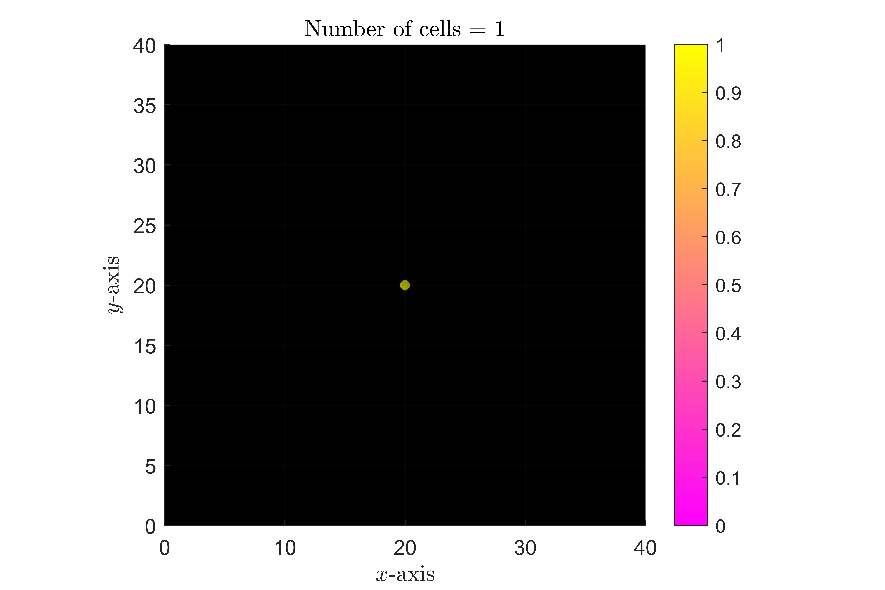
\includegraphics[width=1\textwidth]{chapter1/figures/ColonySimulationDemo_N_1.pdf}
\caption{A starting configuration consisting of a cell with radius $1$ unit equals $3.5 \mu m$}
\label{fig:ColonySimulationStartingCell}
\end{figure}
\filbreak


\begin{figure}[h]
\centering
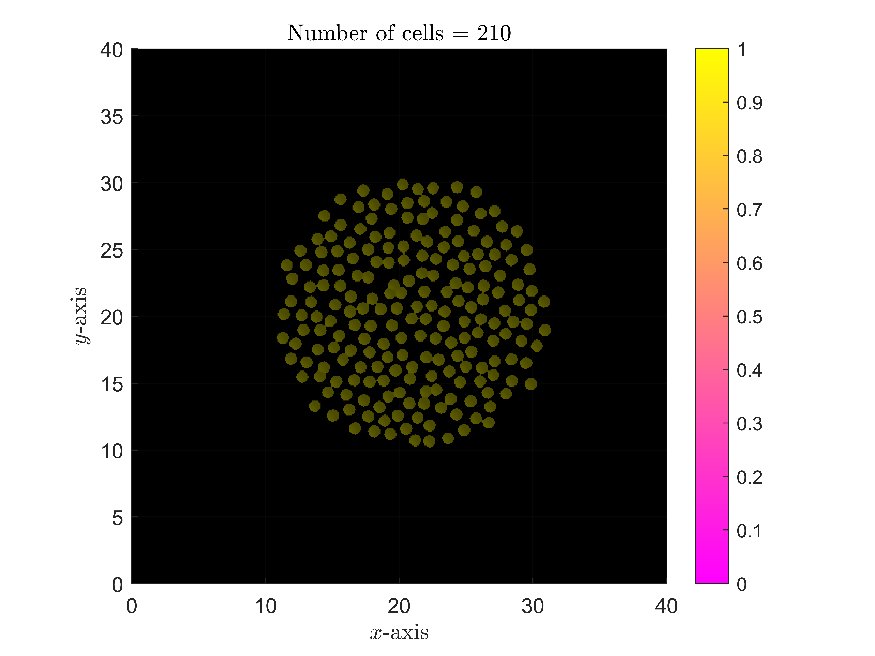
\includegraphics[width=1\textwidth]{chapter1/figures/ColonySimulationDemo_N_210.pdf}
\caption{The same colony at 210 cells}
\label{fig:ColonySimulationN210}
\end{figure}
\filbreak

\section{Adding in a nutrient field}


\begin{figure}[h]
\centering
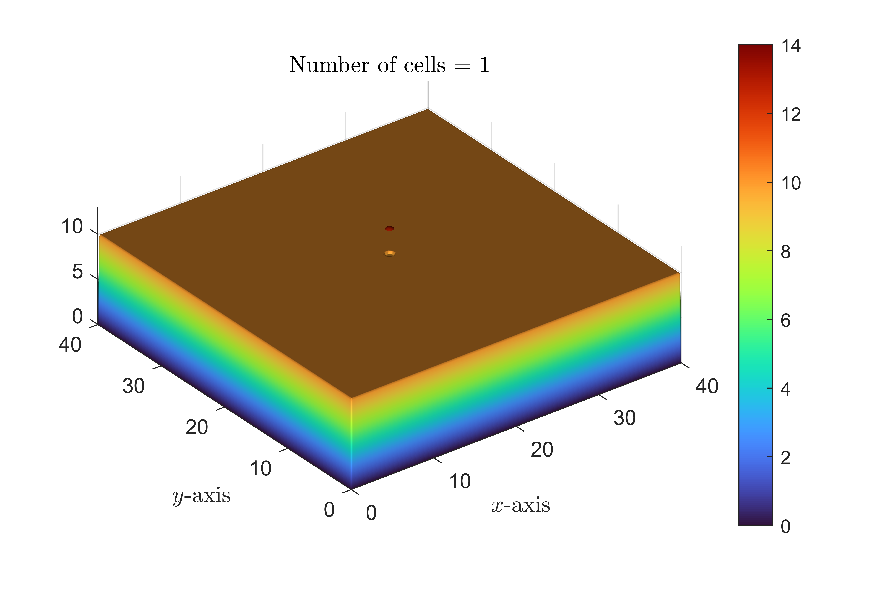
\includegraphics[width=1\textwidth]{chapter1/figures/ColonySimulationDemoNutrientField_N_1.pdf}
\caption{A starting configuration consisting of a cell with radius $1$ unit equals $3.5 \mu m$}
\label{fig:ColonySimulationStartingCellNutrientField}
\end{figure}
\filbreak


\begin{figure}[h]
\centering
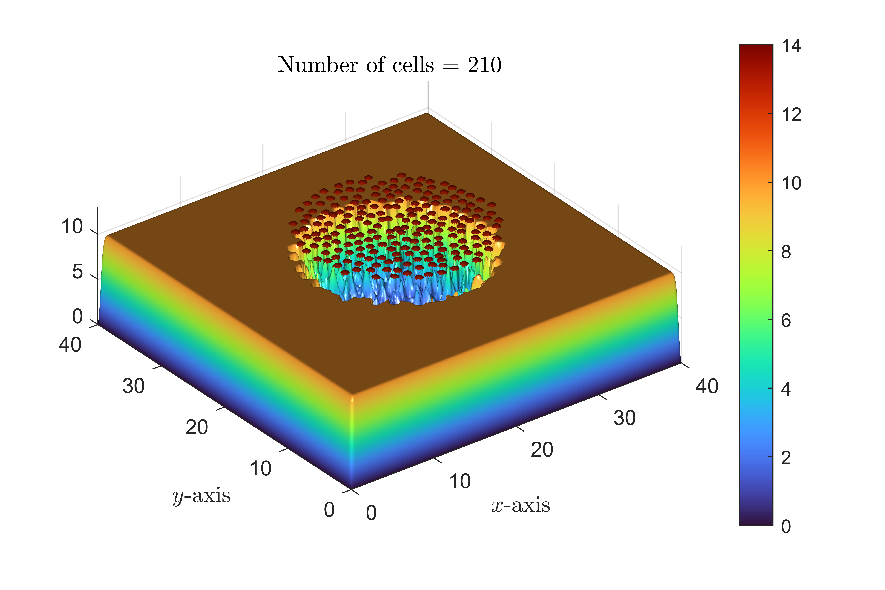
\includegraphics[width=1\textwidth]{chapter1/figures/ColonySimulationDemoNutrientField_N_210.pdf}
\caption{The same colony at 210 cells}
\label{fig:ColonySimulationNutrientFieldN210}
\end{figure}
\filbreak

\section{Simulating $N > 1000$ cells with a nutrient field}

Explain how I have used hash mapping to deal with cell collisions.

\begin{figure}[!htb] %Change this to [p] maybe ?
\centering
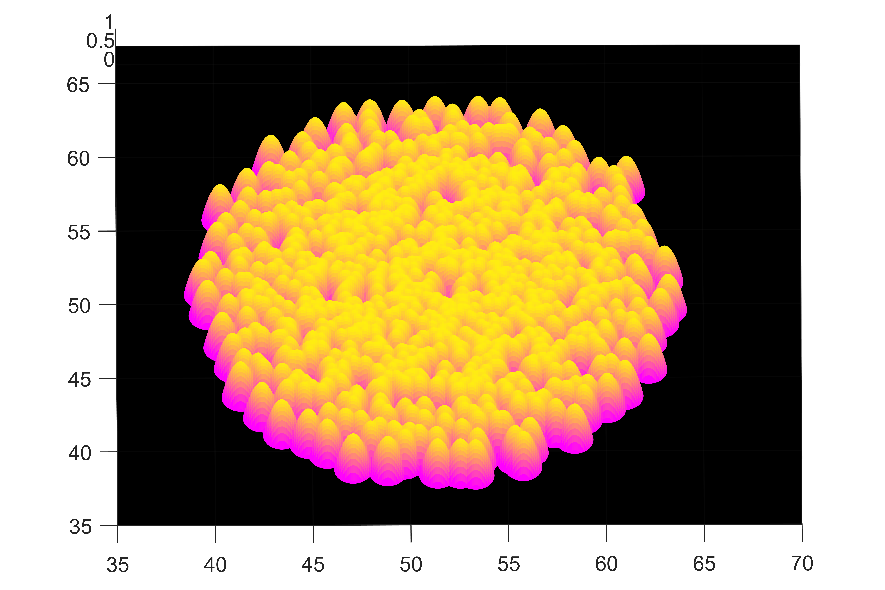
\includegraphics[width=1\textwidth]{chapter1/figures/ColonySimulationDemoNutrientField_N_1065.pdf}
\caption{A cell colony with 1065 cells }
\label{fig:ColonySimulationNutrientFieldN210}
\end{figure}
\filbreak



\section{Calculating the compactness metric}
A fully grown colony will in general not be perfectly circular in shape. In order to measure the roundness of the colony we use the metric used for roundness in image processing
\begin{equation}
    \Psi = \frac{P^2}{4 \pi A},
\end{equation}
where $\Psi \in [0,1]$ is $1$ for a perfect circle and can get to $0$ for highly non-round shapes, $A$ is the colony area, and $P$ is the colony perimeter. When the cells are undergoing mitosis, we are left with the issue of calculating roundness of the blended ``pill" shape geometry of two cells right before splitting. In affect, it will be necessary to calculate the length of 


\section{Collision Detection}

\begin{figure}
    \centering
    \begin{tikzpicture}


    
    \draw[->] (0,0) -- (3,0) node[right] {$x$};
    \draw[->] (0,0) -- (0,3) node[above] {$y$};
    \draw (0,0) circle (0.2);

    % Mass points and rod
    \draw[thick] (4,1) -- (8,2);

    % Mass m1
    \fill (4,1) circle (2pt) node[left] {$m_1$};
    % Mass m2
    \fill (8,2) circle (2pt) node[right] {$m_2$};

    % Center of mass
    \draw[fill=none] (6,1.5) circle (3pt);
    \node at (6.3,1) {$O_C$};

    % Distance markers
    \draw[<->] (4,1.2) -- (6,1.7) node[midway, above] {$d$};
    \draw[<->] (6,1.7) -- (8,2.2) node[midway, above] {$d$};

\end{tikzpicture}
    \caption{Shows a rod shaped backbone of an elliptical cell made from two masses $m_1 = m_2 = m$ connected by a massless rod of length $2d$}
    \label{fig:rod}
\end{figure}



\begin{figure}
    \centering
    \begin{tikzpicture}
    
    % Axes
    \draw[thick,->] (-1,0) -- (5,0) node[right] {$x$};
    \draw[thick,->] (0,-1) -- (0,5) node[above] {$y$};
    \draw[thick] (0,0) circle (0.15); % Rotational point

    % Rod
    \draw[thick]  (1,1) -- (4,3);
    
    % Points on the rod
    \fill (1,1) circle (0.07) node[below left] {1};
    \fill (4,3) circle (0.07) node[above right] {2};

    
    
    % Center of mass
    \draw[thick] (2.5,2) circle (0.15) node[right] {$O_C$};x

    %Center of action of force
    \fill (3.25,2.5) circle (0.07) node[above right] {P};

    % Forces
    \draw[->,thick] (3.25,2.5) -- ++(1,0.66667) node[above right] {$F_t$};
    \draw[->,thick] (3.25,2.5) -- ++(0,1.5) node[above] {$F$};
    \draw[->,thick] (3.25,2.5) -- ++(-0.8,1.2) node[left] {$F_n$};
    
    % Tangent and normal directions
    \draw[dashed] (4,3) -- ++(3,2) node[right] {$t$};
    \draw[dashed] (2.5,2) -- ++(-2,3) node[left] {$n$};

    %extra line for angle
    \draw[dashed] (1,1) -- ++(1.0,0)  node[right]{} ;

    % Angles
    %\draw[->] (1,1) ++(0.3,0.1) arc (0:30:0.3) %node[right] {$\theta_C$};
    %\draw[->] (2.5,2) ++(0.3,0.1) arc %(0:30:0.3) node[right] {$\theta_C$};

    \coordinate (A) at (1,1);
    \coordinate (B) at (1.5,1);
    \coordinate (C) at (1.416,1.2774);

    \draw pic["$\theta_C$",draw=green,<->,angle eccentricity=1.2,angle radius=1cm] {angle=B--A--C};

 
    \end{tikzpicture}
    \caption{Shows a rod shaped cell which is being impinged upon by a contact force $\vb{F}$ resolved into a tangential $F_t$ and normal component $F_n$.}
    \label{fig:rod_force}
\end{figure}

Referring to the supplied figures, we see that a force is $\vb{F}$ in Figure \ref{fig:rod_force} can be a representation of an applied force from another cell acting on the current cell. We set out to find forces on the two point mass that will produce equivalent force balance in the $(t,n)$ coordinate system.

We replace the force $\vb{F}$ with $\vb{F}_1$ and $\vb{F}_2$ acting on mass $1$ and $2$, respectively. From force balance
\begin{equation*}
 \vb{F}_1+  \vb{F}_2 = \vb{F}, 
\end{equation*}
and, from moment balance with anti-clockwise positive,
\begin{equation*}
 l_F F_n = d(F_{2,n} - F_{1,n}).
\end{equation*}
In our case, the impinging force will be from another cell, so we start by making the assumption that there is no tangential force, i.e. frictionless slipping. With this we can
derive simultaneous equations for $F_{1,n}$ and $F_{2,n}$ which have the solution
\begin{equation*}
    F_{1,n} =  \left( \frac{d-l_F}{2d} \right) F_n,
\end{equation*}

\begin{equation*}
    F_{2,n} =  \left( \frac{d+l_F}{2d} \right) F_n.
\end{equation*}
Assuming, once again, that $F_{1,t} = F_{2,t} = F_t = 0$ we can obtain the $(x,y)$ components by doing a coordinate transformation by the angle $-\theta_C = - \arctan{\left( y_2-y_1, x_2-x_1  \right)}$ where $(x_1,y_1)$ and $(x_2,y_2)$ are the mass positions, respectively. So, we have that the components of the force are given by 
\begin{equation*}
    \begin{bmatrix}
    F_{1,x} \\
    F_{1,y} 
    \end{bmatrix}
    =
    \begin{bmatrix}
    \cos{(-\theta_C)} & -\sin{(-\theta_C)}\\
    \sin{(-\theta_C)} & \cos{(-\theta_C)} 
    \end{bmatrix}
    \begin{bmatrix}
    -F_{1,n} \\
    0 
    \end{bmatrix}
    =
    \begin{bmatrix}
    \cos{\theta_C} & \sin{\theta_C}\\
    -\sin{\theta_C} & \cos{\theta_C} 
    \end{bmatrix}
    \begin{bmatrix}
    -\left( \frac{d-l_F}{2d} \right) F_n \\
    0 
    \end{bmatrix},   
\end{equation*}



\begin{equation*}
    \begin{bmatrix}
    F_{2,x} \\
    F_{2,y} 
    \end{bmatrix}
    =
    \begin{bmatrix}
    \cos{(-\theta_C)} & -\sin{(-\theta_C)}\\
    \sin{(-\theta_C)} & \cos{(-\theta_C)} 
    \end{bmatrix}
    \begin{bmatrix}
    F_{2,n} \\
    0 
    \end{bmatrix}
    =
    \begin{bmatrix}
    \cos{\theta_C} & \sin{\theta_C}\\
    -\sin{\theta_C} & \cos{\theta_C} 
    \end{bmatrix}
    \begin{bmatrix}
    \left( \frac{d+l_F}{2d} \right) F_n \\
    0 
    \end{bmatrix}.    
\end{equation*}
We solve this as
\begin{equation*}
  \vb{F}_1 =  - \left(\frac{d-l_F}{2d} \right)  F_n \cos{\theta_C} \hat{\vb{i}} + \left(\frac{d-l_F}{2d} \right)  F_n \sin{\theta_C} \hat{\vb{j}},
\end{equation*}

\begin{equation*}
  \vb{F}_2 =   \left(\frac{d+l_F}{2d} \right)  F_n \cos{\theta_C} \hat{\vb{i}} - \left(\frac{d+l_F}{2d} \right)  F_n \sin{\theta_C} \hat{\vb{j}},
\end{equation*}

\section{Approximate Bayesian Computation (ABC) for the inverse problem}
The traditional statement of Bayes' Theorem goes like
\begin{equation}
    P(A | B) = \frac{P(B|A) P(A)}{P(B)},
\end{equation}
where $A$ and $B$ are outcomes and the terms are given by
\begin{itemize}
    \item $P(A | B)$ is the posterior probability; the probability of $A$ given $B$,
    \item $P(B|A)$ is the conditional probability
    \item $P(A)$ is the prior probability; probability of observing event $A$
    \item $P(B)$ is the marginal probability; probability of observing event $B$
\end{itemize}








